%Results
\section{Descriptive statistics}
Before the experiment, the seeds were weighted in groups of ten, to see if there was a baseline difference between certain genotypes. Table \ref{tab:germination_percentage}, in the previous section, displays the measured weights.
After the completion of the experiment, the outliers were identified, and each plant was attributed a specific weight, following the protocol described in material and methods section. Those weights were used to compute the weighted mean and weighted standard deviation of the fresh and dry weight of the root system and the leaf system, as well as the area of the root system, for each plant. Dotplots representing those descritptive statistics as well as the data point are presented in figure \ref{fig:dotplot_all_variables}. The numerical values of these results are presented in table \ref{tab:summary_table_all_variables}, in appendix \ref{appendix:mean_std_table}.\\

Even though no clear conclusions can be made from these figures, we can see large variation of mean values between genotypes. Also, for some genotypes, the difference between tanks seem significant (e.g. genotype 15) while it's clearly not the case for some other (e.g. genotype 7). This implies that the tank and genotypes effects are significant. Overall the values of dry weights seem to have less variations than the fresh weights.

\begin{figure}
\centering
	\begin{subfigure}[t]{\textwidth}
		\centering
		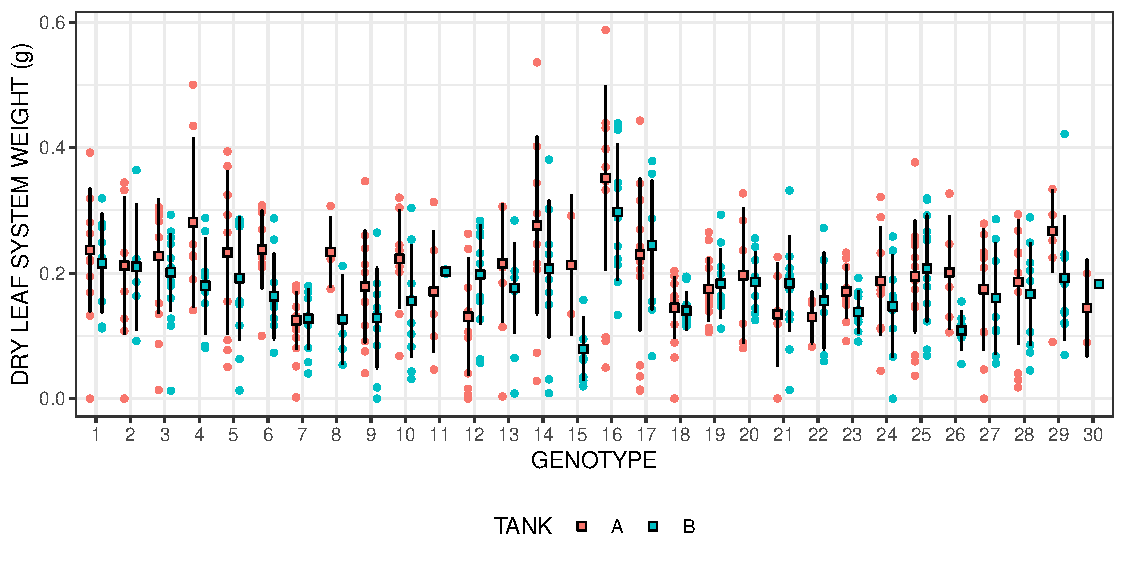
\includegraphics[width = \textwidth]{../../Figures/DRY_LS_summary_plot.pdf}
		\caption{Dry leaf weight ($DRY\_LS$)}
	\end{subfigure}

	\begin{subfigure}[t]{\textwidth}
		\centering
		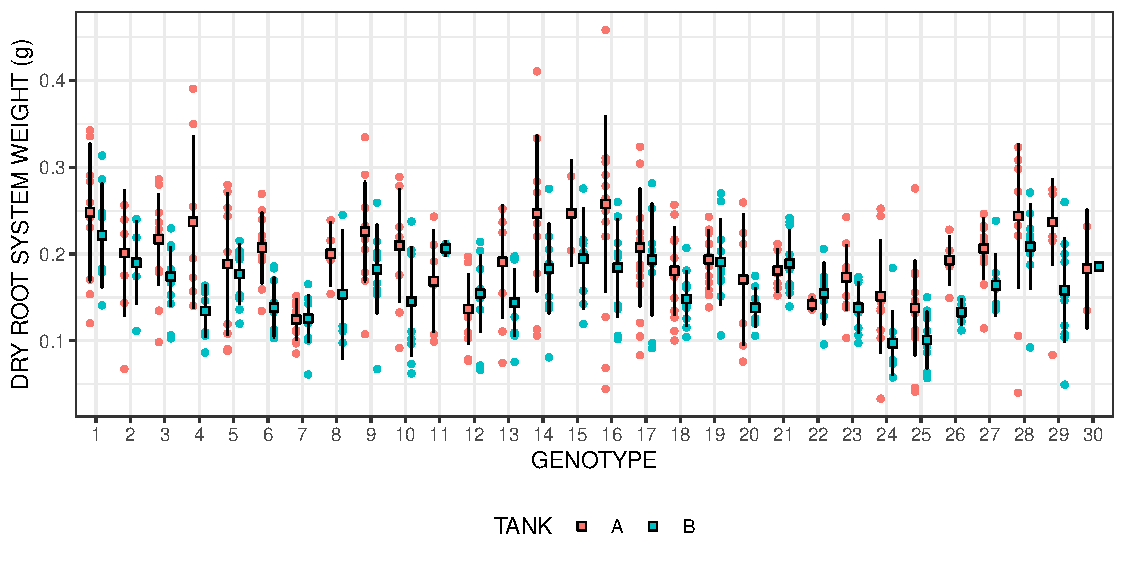
\includegraphics[width = \textwidth]{../../Figures/DRY_RS_summary_plot.pdf}
		\caption{Dry root weight ($DRY\_RS$)}
	\end{subfigure}
	\caption[Dotplot of the mean weight and associated standard deviation]{Dotplot displaying mean weight (\protect\emptysquare) and associated standard deviation (\protect\blackline), grouped by tanks for each variable.}
\end{figure}
\begin{figure}\ContinuedFloat
	\captionsetup[figure]{list=no}
	\begin{subfigure}[t]{\textwidth}
		\centering
		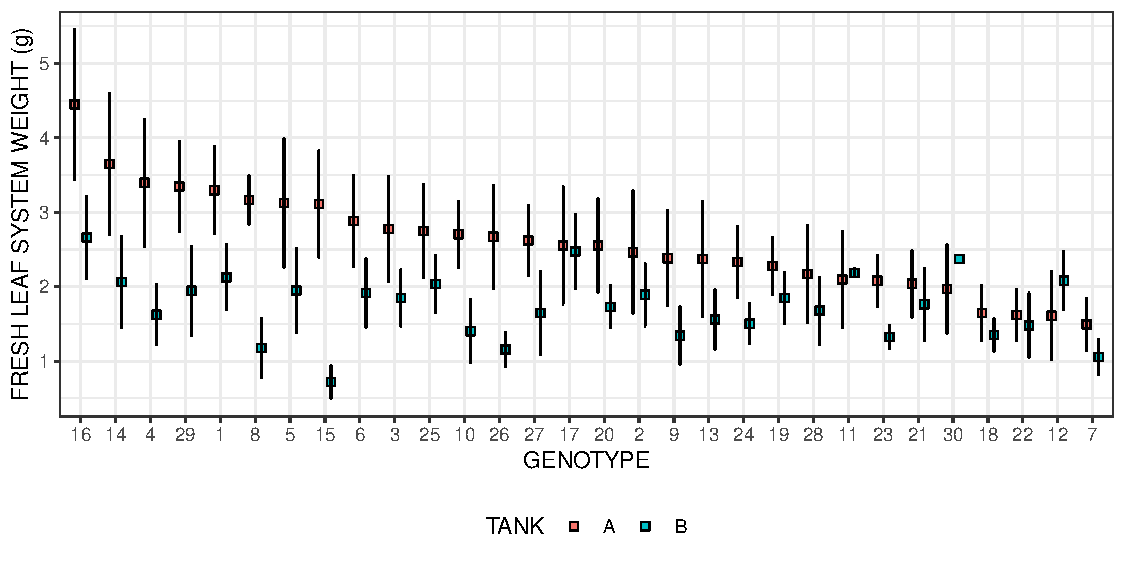
\includegraphics[width = \textwidth]{../../Figures/FRESH_LS_summary_plot.pdf}
		\caption{Fresh leaf weight ($FRESH\_LS$)}
	\end{subfigure}

	\begin{subfigure}[t]{\textwidth}
		\centering
		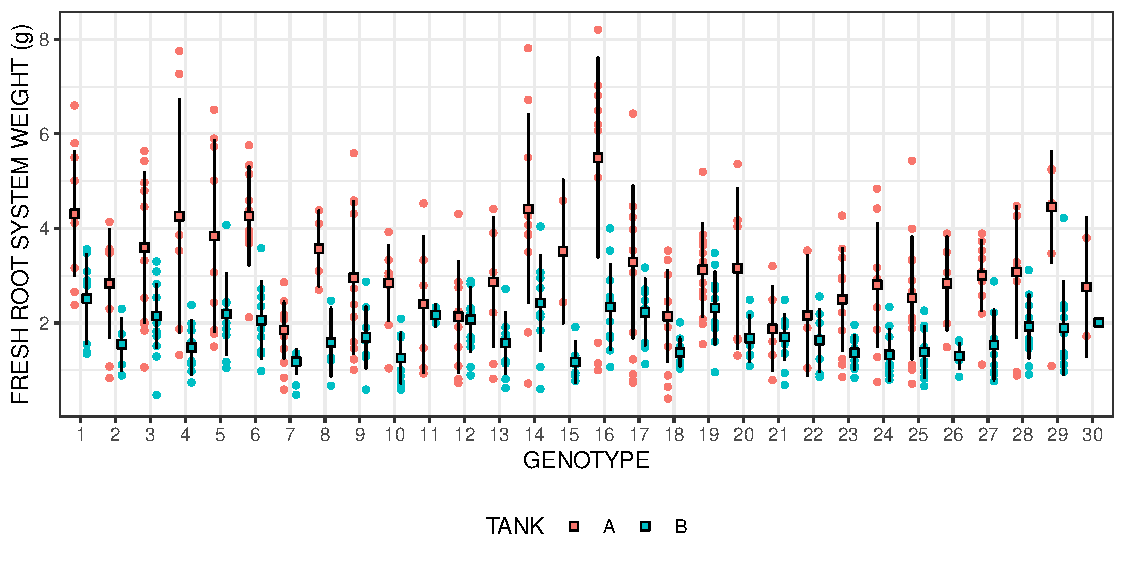
\includegraphics[width = \textwidth]{../../Figures/FRESH_RS_summary_plot.pdf}
		\caption{Fresh root weight ($FRESH\_RS$)}
	\end{subfigure}
	\caption[Dotplot of the mean weight and associated standard deviation]{Dotplot displaying mean weight (\protect\emptysquare) and associated standard deviation (\protect\blackline), grouped by tanks for each variable.}
	\label{fig:dotplot_all_variables}
\end{figure}

\section{SpATS analysis}
The SpATS model usually takes rows and columns coordinates as inputs for spatial position. Given that we have tanks (A and B), strips (from 1 to 99) and positions (from 1 to 5), we reshaped the data to give have the tank side by side and the 99 strips divided in two columns (to have a similar disposition to the one in the greenhouse). Figure \ref{fig:tank_disposition} shows the reshaping of the positions. This new display of the data allows us to see the difference between tanks more clearly and to visualize the variables' values as they were in the greenhouse.

\begin{figure}[hbtp]
	\centering
	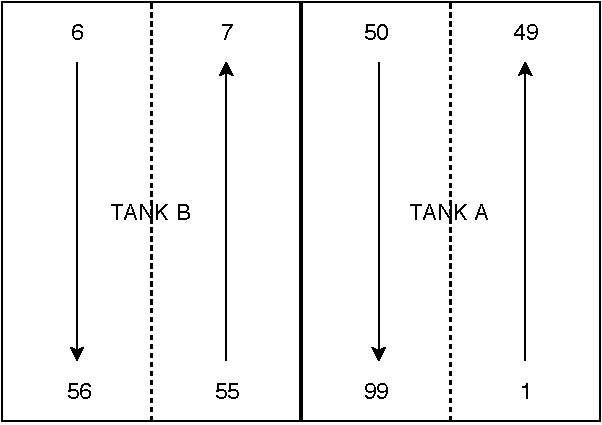
\includegraphics[scale = 0.7]{figures/TANK_repartition.pdf}
	\caption[Reshaping of the data table to fit the disposition of the greenhouse]{Reshaping of the data table to fit the 
	disposition of the greenhouse. The number indicates the original strip number.}
	\label{fig:tank_disposition}	
\end{figure}

The model was then fitted for the four weight variables, using the settings specified in the previous chapter. Table \ref{tab:spats_dimensions} presents the effective dimensions associated with the bivariate smooth surface components (see equation \ref{eq:full_bivariate_smooth_surface_model}) 
and their relative contribution to the fitted surface for each variable.
We see that the fresh weights exhibited a higher complexity in the structure of the spatial surface. This is reflected by the higher value of contribution for the smooth-by-smooth term ($f_{u, v}(\boldsymbol{u}, \boldsymbol{v})$), that accounts for almost 70\% in both variables. Besides this term, the main sources of variation are the linear (for the strips) by smooth (for the positions) term and the smooth trend along the strips term. It is not surprising to have more variation along the strips than along the positions given that there were 99 strips but only 5 positions.
Concerning the dry weights, the variation is more spread between all the components for both variables. This means that the variation in the data can be more easily attributed to the strips and positions of the plants. However, all the variables have component with zero value of $ED_{s}$ (the actual values were not zero but it is denoted as such since they were inferior to $1 \times 10^{-15}$), indicating that these terms were not necessary to model the spatial surface.\\



% Table generated by Excel2LaTeX from sheet 'Sheet2'
\begin{table}[htbp]
  \rowcolors{2}{gray!25}{white}
  \centering
  \caption[Effective dimensions of the SpATS model]{Model dimensions and effective dimensions (and percentage of the total of 
  the spatial components) of each spatial components for all variables. $ED_{\epsilon}$ represents the effective dimensions for 
  the residuals; $ED_{g}$, is the effective dimensions for the genotype and $H_{g}^2$ is the heritability. Here $\mathbf{v}$ 
  represents the columns, i.e. the position on the strip; and $\mathbf{u}$ represents the rows, i.e. the strip itself.}
    \begin{tabular}{lrrrrr}
    \toprule
    \begin{tabular}[b]{@{}l@{}}Model \\ components\end{tabular} & \multicolumn{1}{c}{Model} & \multicolumn{1}{l}{FRESH\_LS} & \multicolumn{1}{l}{FRESH\_RS} & \multicolumn{1}{l}{DRY\_LS} & \multicolumn{1}{l}{DRY\_RS} \\
    \midrule
    $f_{v}(\mathbf{v})$ & 6     & 0 (0,00\%) & 0 (0,00\%) & 0 (0,00\%) & 0 (0,00\%) \\
    $f_{u}(\mathbf{u})$ & 100   & 0,8 (8,73\%) & 2,26 (14,10\%) & 1,02 (17,26\%) & 1,8 (17,26\%) \\
    $\boldsymbol{u} \odot h_{v}(\boldsymbol{v})$ & 6     & 1,84 (19,95\%) & 2,63 (16,40\%) & 1,47 (24,77\%) & 2,54 (24,77\%) \\
    $\boldsymbol{v} \odot h_{u}(\boldsymbol{u})$ & 100   & 0,24 (2,56\%) & 0 (0,00\%) & 1,09 (18,36\%) & 0,49 (18,36\%) \\
    $f_{u, v}(\boldsymbol{u}, \boldsymbol{v})$ & 150   & 6,33 (68,76\%) & 11,16 (69,50\%) & 2,35 (39,62\%) & 0,08 (39,62\%) \\
    Total & 362 & 9,21 (100\%) & 16,15 (100\%) & 5,93 (100\%)& 4,91 (100\%)\\
    \midrule
    $ED_{\epsilon}$ &       & 466.6 & 459,3 & 470,2 & 470,1 \\
    \midrule
    $ED_{g}$  & 30    & 21,02 & 22,58 & 21,38 & 22,98 \\
    $H_{g}^2$ &       & 0,72  & 0,78  & 0,74  & 0,79 \\
    \bottomrule
    \end{tabular}%
  \label{tab:spats_dimensions}%
\end{table}%

Figure \ref{fig:spats_model_results} presents the results of the SpATS model.

\begin{figure}
	\begin{subfigure}[t]{\textwidth}
		\centering
		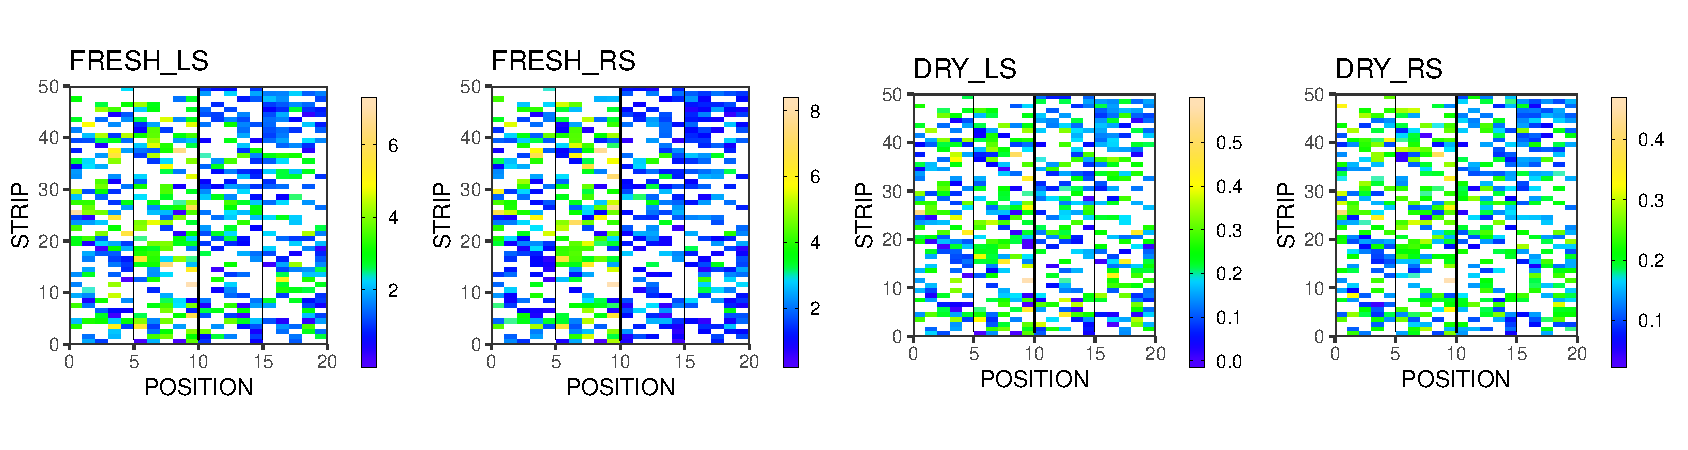
\includegraphics[width = \textwidth]{../../Figures/rawData_plot.pdf}
		\caption{Raw data}
	\end{subfigure}
	
	\begin{subfigure}[t]{\textwidth}
		\centering
		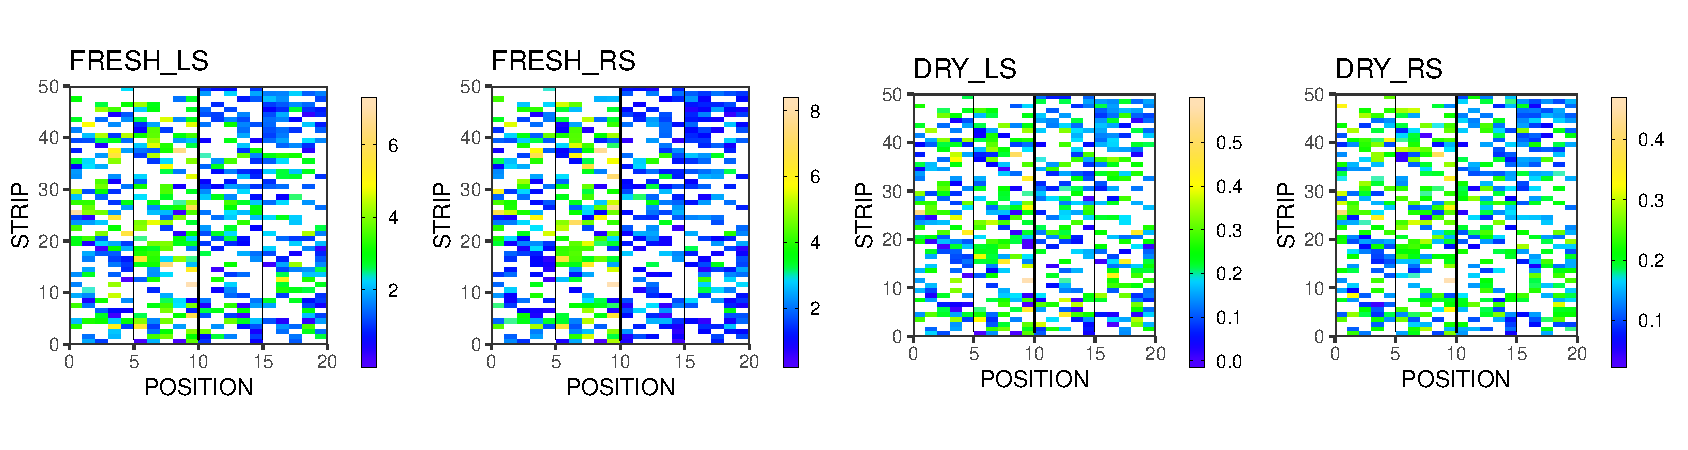
\includegraphics[width = \textwidth]{../../Figures/rawData_plot.pdf}
		\caption{Raw data}
	\end{subfigure}
	
	\begin{subfigure}[t]{\textwidth}
		\centering
		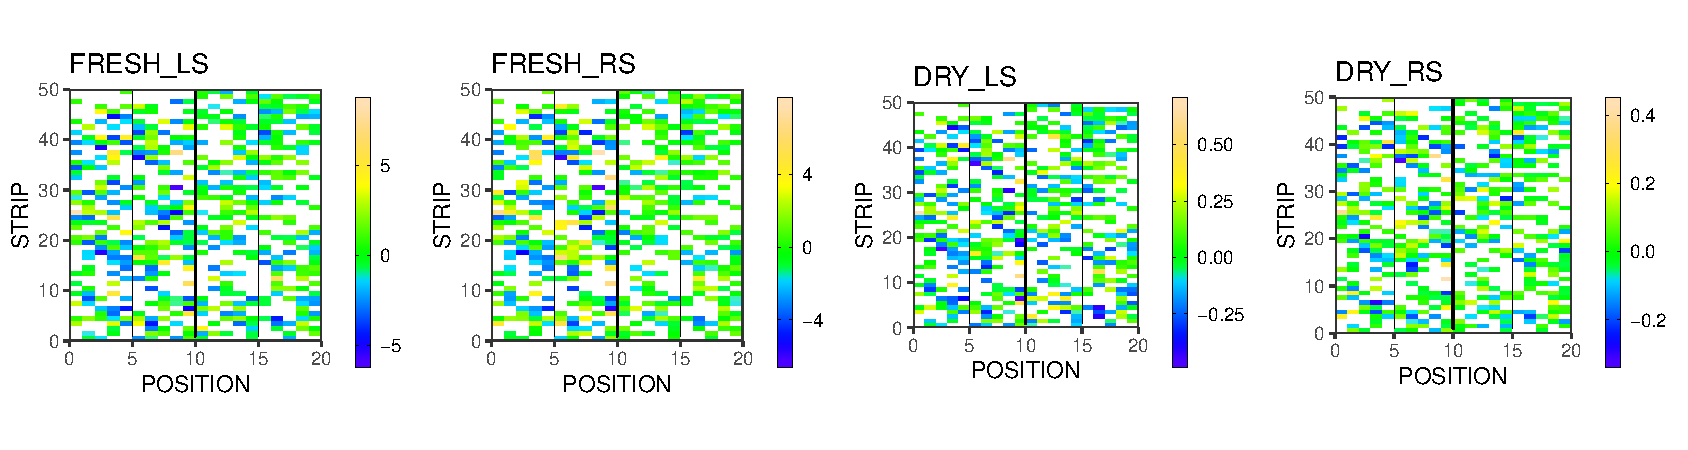
\includegraphics[width = \textwidth]{../../Figures/residuals_plot.pdf}
		\caption{Residuals' spatial plot}
	\end{subfigure}
	\caption{Raw data; fitted spatial trend and residuals' plot for each variable.}
	\label{fig:spats_model_results}
\end{figure}

The plot for the analysis of the residuals are presented on figure \ref{fig:residuals_analysis_plot} in appendix \ref{appendix:residuals}.

\section{ARxAR model analysis}
\section{Model comparison}
\subsection{Performances}
\subsection{Parametrization}
\subsection{Modelling strategy}
